\documentclass{article}

% Language setting
% Replace `english' with e.g. `spanish' to change the document language
\usepackage[english]{babel}

% Set page size and margins
% Replace `letterpaper' with `a4paper' for UK/EU standard size
\usepackage[a4paper,top=2cm,bottom=2cm,left=3cm,right=3cm,marginparwidth=1.75cm]{geometry}

% Useful packages
\usepackage{amsmath}
\usepackage{graphicx}
\usepackage[colorlinks=true, allcolors=blue]{hyperref}
\usepackage{xcolor}
\usepackage{listings}

\colorlet{mygray}{black!30}
\colorlet{mygreen}{green!60!blue}
\colorlet{mymauve}{red!60!blue}

\lstdefinelanguage{cpp}{
  backgroundcolor=\color{gray!10},  
  basicstyle=\ttfamily,
  columns=fullflexible,
  breakatwhitespace=false,      
  breaklines=true,                
  captionpos=b,                    
  commentstyle=\color{mygreen}, 
  extendedchars=true,              
  frame=single,                   
  keepspaces=true,             
  keywordstyle=\color{blue},      
  language=c++,                 
  numbers=none,                
  numbersep=5pt,                   
  numberstyle=\tiny\color{blue}, 
  rulecolor=\color{mygray},        
  showspaces=false,
  showstringspaces=false,
  showtabs=false,                 
  stepnumber=5,                  
  stringstyle=\color{mymauve},    
  tabsize=3,                                     
  title=\lstname 
}
\lstset{language=cpp}
\lstnewenvironment{code}[2][]{%
  \lstset{%
    numbers = left,
    title   = #2,
    #1,
  }%
}{}

\title{Assignment 2.1}
\author{Steinarr Hrafn Höskuldsson}

\usepackage{fancyhdr}
\fancypagestyle{firststyle}
{
   \fancyhf{}
   \fancyhead[L]{Embedded Systems Programming}
   
   \renewcommand{\headrulewidth}{0pt} % removes horizontal header line
}

\newcommand{\mycomment}[1]{}
\begin{document}
\pagestyle{firststyle}
{\let\newpage\relax\maketitle}

\mycomment{
\begin{figure}[h]
    \centering
    \includegraphics[width=0.75\textwidth]{LAB3/Basic1.png}
    \caption{"Switch test" Breadboard set up}
    \label{fig:Switch_test}
\end{figure}

\lstinputlisting[caption=Defining 'ColorMatch' state, label={lst:colormatch}, language=Python, firstline=44, lastline=52]{LAB3/Basic.py}

}

\section*{Part 1}
A new project was created in PlatformIO and a use case diagram using plantUML was written. 

\lstinputlisting[caption=state.wsd]{Assignment3_2TestDrivenDevelopment/docs/diagrams/src/use_case.plantuml}

Which generated the following diagram:
\begin{figure}[h]
    \centering
    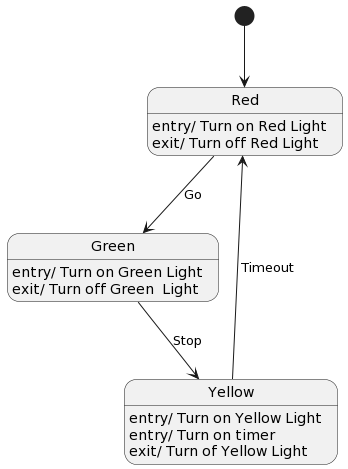
\includegraphics[width=0.5\textwidth]{Assignment3_1StateBehaviour/docs/diagrams/fsm2.png}
    \caption{Finite State Machine Diagram of a simplified traffic light.}
\end{figure}

\section*{Part 2}
The state machine was implemented using a switch case setup. The code can be seen in appendix \ref{appendix:code}.
\mycomment{
\begin{figure}[h]
    \centering
    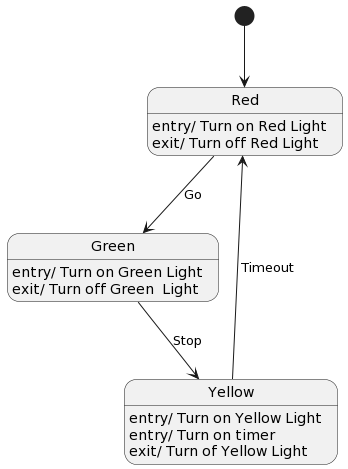
\includegraphics[width=0.5\textwidth]{Assignment3_1StateBehaviour/docs/diagrams/fsm2.png}
    \caption{Updated Finite State Machine Diagram of a simplified traffic light.}
\end{figure}
}
Running the code resulted in the following behaviour, note that lines encased in \{\} are comments added afterwards.

\lstset{language=}
\begin{lstlisting}
Part 2, State Machine, based on Refactoring Gurus example
RedLight->ON

{sending: g}

I received: 103
I received a go command
RedLight->OFF
GreenLight->ON

{sending s}

I received: 115
I received a stop command
GreenLight->OFF
YellowLight->ON

{there was a delay here}

YellowLight->OFF
RedLight->ON
\end{lstlisting}
\lstset{language=cpp}


\section*{Part 3}
The State behaviour was implemented based on the example from Reference Guru. The Context and State Definitions were moved to Context.h and each class definition was moved into its own header file.
Here is the program. All relevant header files can be seen in Appendix \ref{appendix:code}
\lstinputlisting[caption=main.cpp in Part 3]{Assignment3_1StateBehaviour/src/main_prt3.cpp}
The behaviour when run was exactly the same as an be seen in Part 2. 

\newpage
\appendix
\section{Code}\label{appendix:code}

%\lstinputlisting[caption=main.cpp in Part 2]{Assignment3_1StateBehaviour/src/main_prt2.cpp_old}

\lstinputlisting[caption=Context.h]{Assignment3_1StateBehaviour/src/Context.h}
\lstinputlisting[caption=Red.h]{Assignment3_1StateBehaviour/src/Red.h}
\lstinputlisting[caption=Green.h]{Assignment3_1StateBehaviour/src/Green.h}
\lstinputlisting[caption=Yellow.h]{Assignment3_1StateBehaviour/src/Yellow.h}



% TODO: put these in columns next to each other?

\end{document}

